\documentclass[12pt,a4paper]{scrartcl}
\usepackage[utf8]{inputenc}
\usepackage[english]{babel}
\usepackage{graphicx}
\usepackage{csquotes}
\graphicspath{ {images/} }
\usepackage{float}
\floatplacement{figure}{H}
\usepackage{alltt}
\usepackage{setspace}
\doublespacing
%\usepackage{setspace}
%\setstretch{1.5}
%\expandafter\def\expandafter\quote\expandafter{\quote%\singlespace}
\usepackage[all]{nowidow}
\usepackage{color}
\usepackage{alphalph}
\usepackage[font={small,it}]{caption}
%\usepackage{perpage}
%\MakePerPage{footnote}



\usepackage{lipsum}
\usepackage{filecontents}
\usepackage[dvipsnames]{xcolor}
\usepackage{hyperref}
\usepackage{cleveref}

\newcommand\myshade{85}
\colorlet{mylinkcolor}{violet}
\colorlet{mycitecolor}{YellowOrange}
\colorlet{myurlcolor}{Aquamarine}

\hypersetup{
  linkcolor  = mylinkcolor!\myshade!black,
  citecolor  = mycitecolor!\myshade!black,
  urlcolor   = myurlcolor!\myshade!black,
  colorlinks = true,
}

\renewcommand*{\thefootnote}{\fnsymbol{footnote}}

\setlength{\parskip}{1em}

\author{Sarah Hertz}
\title{Secondary Creations: The Impact of Digital Technology on Publishing}
\subtitle{}
%% remove percentage symbol on line below to remove date
\date{}

\clearpage
\newpage

\addto\captionsenglish{
    \renewcommand*\contentsname{Table of Contents}
}
%\listoffigures

\setcounter{page}{1}

\usepackage[
backend=biber,
style=mla,firstlonghand=false,nofullfootnote=true,
sorting=nty
]{biblatex}

\addbibresource{sample.bib}

\DeclareCiteCommand{\citeauthor}
  {\boolfalse{citetracker}%
   \boolfalse{pagetracker}%
   \usebibmacro{prenote}}
  {\ifciteindex
     {\indexnames{labelname}}
     {}%
   \printtext[bibhyperref]{\printnames{labelname}}}
  {\multicitedelim}
  {\usebibmacro{postnote}}
 

\begin{document}

\begin{titlepage}
\maketitle
\thispagestyle{empty}
\end{titlepage}
\clearpage

\pagenumbering{roman}
\tableofcontents
%\thispagestyle{empty}
\clearpage

\listoffigures
%\thispagestyle{empty}
\clearpage

\clearpage
\pagenumbering{arabic}

\phantomsection
\addcontentsline{toc}{section}{Introduction}
\section*{Introduction}

In 1571, Michel de Montaigne retired from public life to his ‘tower’, where he shut himself away for ten years with some 1,500 books, to work on his \textit{Essais}. Today, he is remembered as one of history's most voracious readers: 

\begin{displayquote}
I seek, in the reading of books, only to please myself by an honest diversion; or, if I study, ‘tis for no other science than what treats of the knowledge of myself, and instructs me how to die and how to live well \autocite{montaigne}.\footnote{\textquote{Je ne cherche aux livres qu'à m'y donner du plaisir par un honneste amusement: ou si j'estudie, je n'y cherche que la science, qui traicte de la connoissance de moy-mesmes, \& qui m'instruise à bien mourir \& à bien vivre}\parencite[91]{french}.}
\end{displayquote}

This passage suggests that although technology has changed since the sixteenth century, the purpose for reading has not. After all, the codex was invented around 300 AD to instruct readers `how to die and how to live well', by Christ's example. During this time, the transition from scroll to codex was instrumental in the dissemination of Christian doctrine. Compared with the scroll, the codex is easier to hold, transport, and store. The Roman poet Martial is allegedly the first to recognize its advantages, asking readers to \textquote{buy these verses, which parchment gets into fewer pages}.\phantomsection\footnote{\textquote{\textit{Hos eme, quos artat brevibus membrana tabellis}.}\parencite[187]{winsbury}.}

`Modern' books emerged with the invention of the printing press in 1440, by Johannes Gutenberg. During the Protestant Reformation, the printing press aided in the democratization of knowledge, with the dissemination of vernacular Bible translations: the first, by Martin Luther, into German; the second, by William Tyndale, into English. Lower production costs made chapbooks and hardbacks more widely accessible. Although the growth is difficult to quantify, scholars estimate that there were eight to twenty million incunabula, or early printed books, by 1500. With so many authors competing for attention, Early Modern readers underwent an `information overload', not unlike our experience of Internet.\footnote{For more on Early Modern and contemporary reading experiences respectively, see \citeauthor{blair} and \citeauthor{jacobs}.} Not only did readers question the authoritativeness of the text, but also the quality of the books themselves, as finished products. Even as late as 1894, J. M. Bowles remarked that \phantomsection\textquote{most people have no ideals at all with regard to printing; there is so little that is good, and the little good there is, is almost lost under the great mass of bad constantly being thrust before them}\parencite{bowles}.

\section{Adaptability}

Perhaps J. M. Bowles would find it comforting that some people still appreciate print aesthetics. Previously the Editorial Director for Raincoast Books, and now the Director of the University of Calgary Press, Brian Scrivener values quality printing, despite economic pressures. As he says, \textquote{publishing is not a profession, publishing is craftwork; it is, in essence, secondary creation} \phantomsection\parencite{scrivener}.\par 

Drawing from a lifetime's experience in trade and scholarly publishing, Brian is using the flexibility of electronic texts to the Press' advantage. As the editors of the \textit{International Journal of American Linguistics} note, the \phantomsection\textquote{web allows publication of supplementary materials and appendixes that are too lengthy to include in the print version of the \textit{Journal}} \parencite[2]{beck}. The inclusion of video and audio files in electronic publications will enhance the reading experience, Brian says. Books that \phantomsection\textquote{update themselves} could benefit biomedical researchers, textbook publishers, and anyone else requiring the latest data \parencite{scrivener}. This, in turn, would increase productivity by reducing production and distribution costs, just as smaller print runs are already viable, thanks to POD.\footnote{Along with Bill Martin, I define `digital publishing' as \textquote{the production and distribution of digital content using the World Wide Web as a communication channel, with provision for the establishment of digital database facilities for future reuse}\cite[39]{martin}.}

The following chart illustrates the many internal and external forces impacting publishing, including globalization, mergers, technological change, and shifting consumer demands and behaviours:

%\clearpage
\phantomsection
%\addcontentsline{toc}{subsection}{\textbf{Fig. 1} \textit{External and Internal Forces}}
\begin{figure}[H]
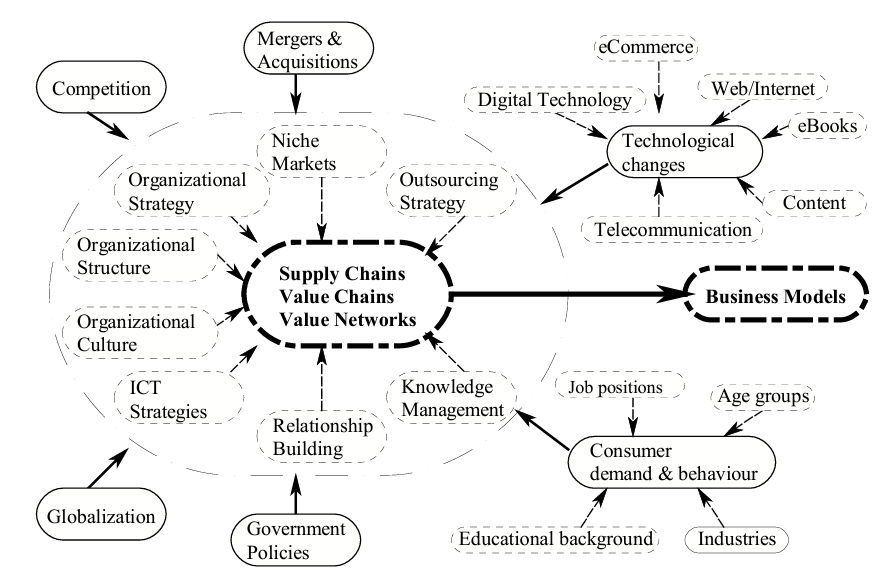
\includegraphics[scale=0.5]{internal}
\centering
\caption{External and Internal Forces}\protect\autocite[18]{martin}
\label{Fig.1}
\centering
\end{figure}

The overarching question, is whether publishers will adapt as quickly as their readers. The cachet of scholarly publishing, Paul Fyfe argues, comes from its correctional and copyediting services:

\begin{displayquote}
Corrected and copyedited texts are saleable and signify in a reputational economy because they have been processed in ways that users are unlikely to replicate or undertake themselves. Correction is the `added value' of publication, part of an increasingly outmoded business plan or a contractual relic of scholarly values that ought to be renegotiated. \autocite[265]{fyfe}
\end{displayquote}

Scholarly publishers ought to reconsider their role, as correctional and copyediting services become automated. By digitizing their frontlists and backlists, making them available OA or POD, and adapting workflow processes, supply chains, digital storage, and distribution, they might stay competitive \autocite[39]{martin}.\footnote{Open Access and Print On Demand, respectively.} Social media marketing can renew interest in older titles, for free. However, `technical obsolescence', such as hardware and browser interoperability, as well as broken links or `link rot', remain challenging aspects of innovation \parencite[260]{fyfe}. 
 
 \section{Accessiblity}

Like the printing press, digital publishing facilitates knowledge dissemination. This is especially relevant to academics, who are more interested in informational content than they are in the materiality of the text (with the exception of Book History scholars). Outreach educational programs, such as Worldreader, bring books to developing countries on Kindles and cell phones.\footnote{For more information, visit
\href{http://www.worldreader.org/}{Worldreader}.} 

Still, every new technology presents an opportunity for censorship. In 1581, Queen Elizabeth I gave Master Edmund Tilney the right to license and censor London plays, including Shakespeare \cite[2]{dutton}.\footnote{Qtd. in Dutton: \enquote{we ordaine \ldots to order and reforme, auctorise and put downe, as shalbe thought meete or unmeete unto himself or his said deputie in that behalf}\autocite[2]{dutton}.} More recently, scholars and politicians have compared China's `digital leapfrog'  with Mao Zedong's `Great Leap Forward', as an attempt to catch up with the \textquote{industrialised world through unorthodox means}\autocite[2]{hughes}. Somewhat paradoxically, the People's Republic of China is encouraging Information and Communications Technologies, while regulating online activities. Some proponents of `digital libertarianism' believe ICTs should go uncensored; however most liberal-democratic states, including Canada and the US, impose taxes on cross-border e-commerce, to secure data and prevent cyber crime \cite[59]{hughes}.\footnote{See Ying Jiang's \textit{Cyber-nationalism in China} for a critique of Western media portrayals of Chinese censorship \autocite{jiang}.} Accessibility, therefore, is always a matter of balance.

\section{Readability}

Digital technology is not only affecting what we read, but how we read it. For instance, we forget that the pen is a technology with `rules' dictating its usage:

%\clearpage
\phantomsection
%\addcontentsline{toc}{subsection}{\textbf{Fig. 2} \textit{How to hold a pen}}
\begin{figure}[H]
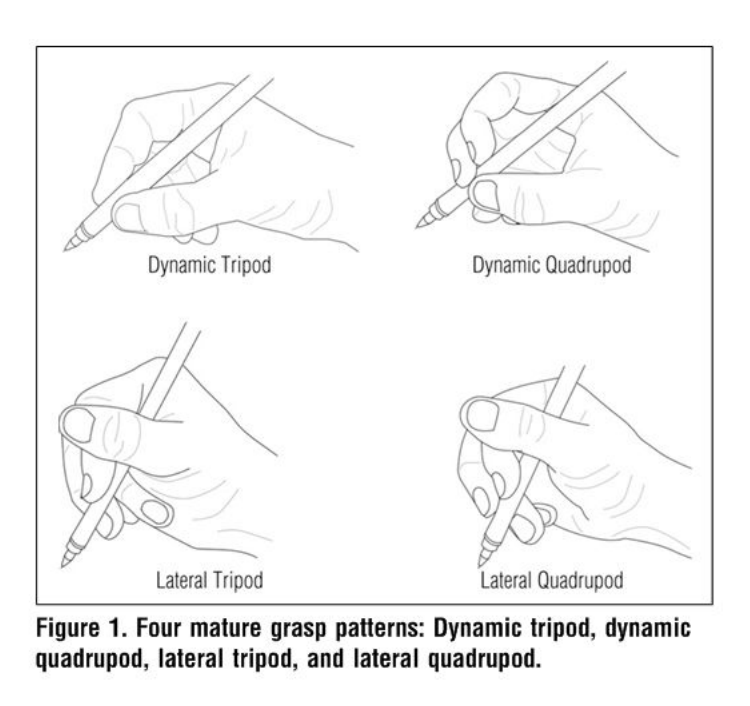
\includegraphics[scale=0.32]{hands}
\centering
\caption{How to Hold a Pen}\protect\autocite[719]{pen}
\label{Fig.2}
\centering
\end{figure}

Unlike the pen or even printed books, there is no established convention for reading ebooks or webpages. Only recently, researchers have found that web users tend to associate the right side of the page with ads, and therefore neglect it \autocite[687]{popa}. Publishing houses and, by extension, marketing administrators ought to consider how and why people read: are they reading slowly for the experience, or skimming for information?

 Not only do today's readers want products, they also expect \textquote{personal attention and contact from publishers and authors, as well as other like-minded readers} \phantomsection\autocite[21]{martin}. Moreover, readers are producing content themselves, through annotation or self-publication. The figure of the lone reader epitomized by Montaigne and Vermeer's \textit{Girl Reading a Letter by an Open Window} might become an historical anomaly:

%\clearpage
\phantomsection
%\addcontentsline{toc}{subsection}{\textbf{Fig. 3} \textit{Girl Reading a Letter by an Open Window}}
\begin{figure}[H]
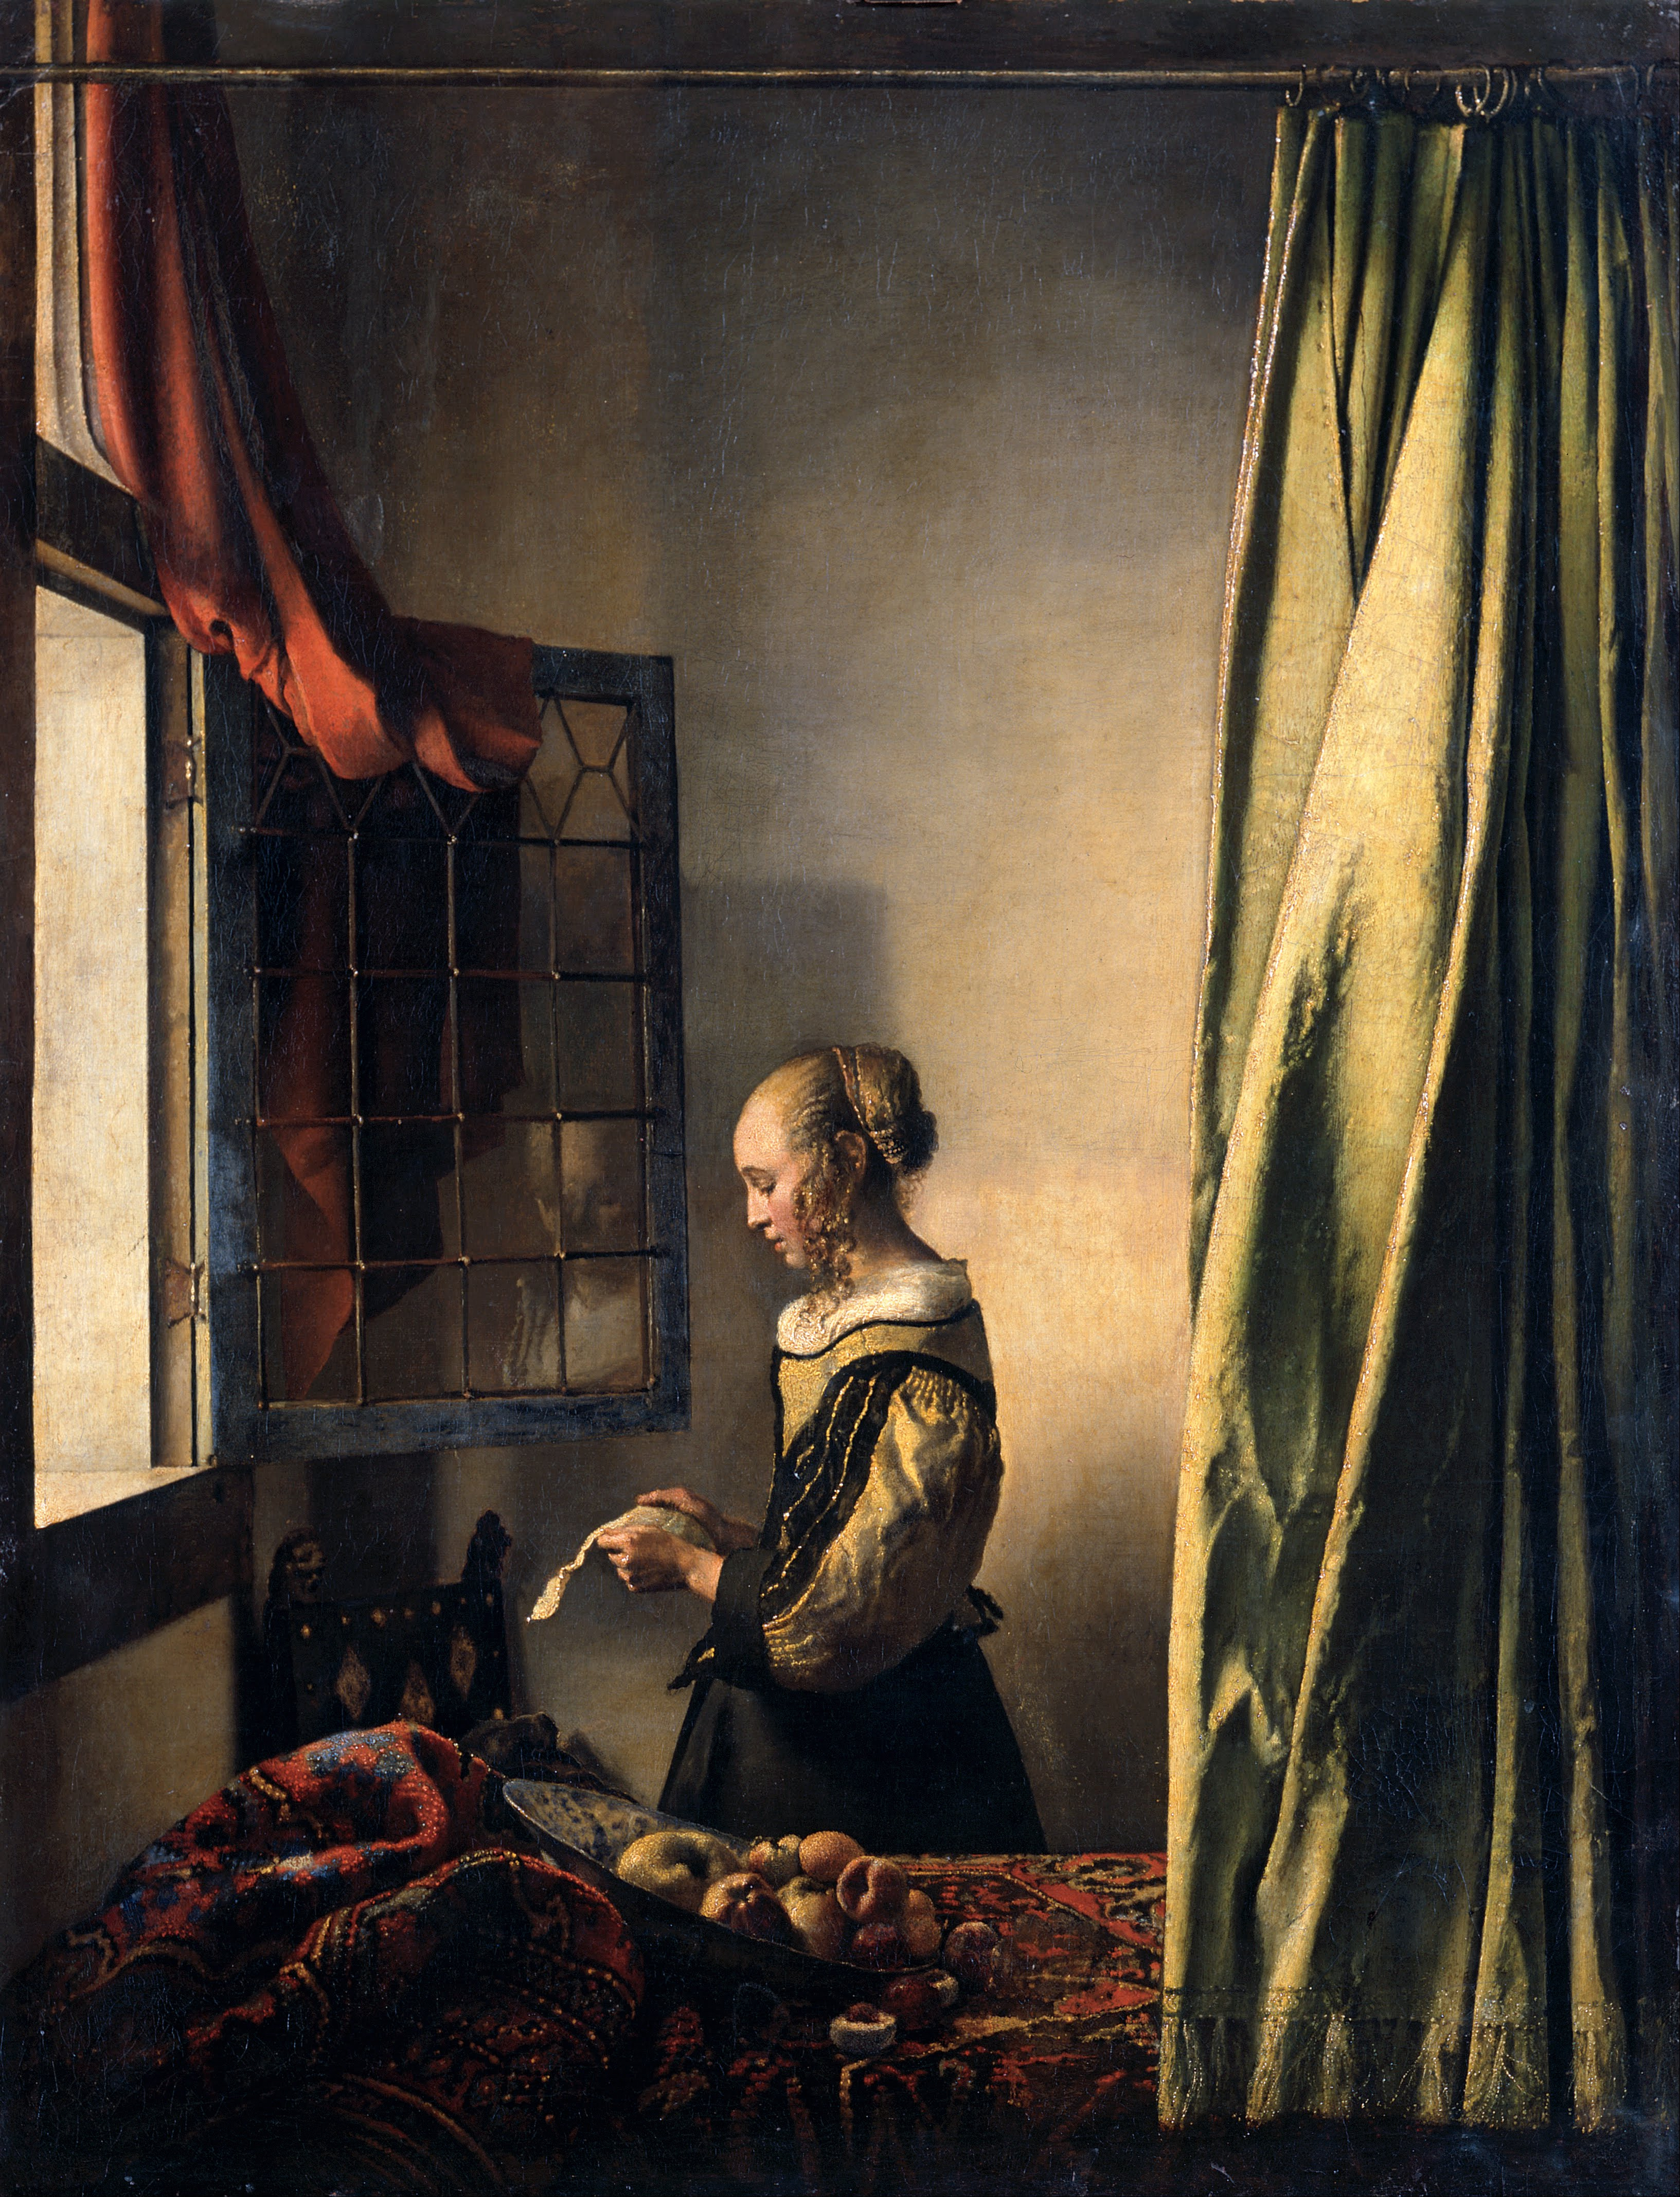
\includegraphics[scale=0.08]{images}
\centering
\caption{\textit{Girl Reading a Letter by an Open Window}}\protect\autocite{vermeer}
\label{Fig.3}
\centering
\end{figure}

How do we define the `book' in the digital age? Are books no longer material objects, but rather `information architectures' or `structured renditions of texts and images'? Or are they places where readers and authors congregate?\phantomsection\footnote{See \citeauthor{martin} and \citeauthor{jacobs} for more on the future of printed books.} If the value in scholarly publishing is not in the correctional and copyediting services it provides, perhaps its purpose is in \textquote{understanding what matters, then gathering the necessary information and disseminating it to those who need it} \cite[39]{martin}.


\clearpage
\phantomsection
\addcontentsline{toc}{section}{References}
\defbibheading{References}{\section*{References}}
\printbibliography[heading=References]

%\BreakBibliography

\end{document}